Эксперименты ставились на парах модельных изображений и на изображениях поверхностях реальных образцов.
\subsection{Образцы изображений}
\subsubsection{Модельные изображения}

В качестве образцов брались наборы изображений из интернет ресурса ``Society for Experimental Mechanics (sem.org)'' описание текстур находится в таблице \ref{tab:set_image}.

\begin{longtable}[h!]{|*7{m{0.12\textwidth}|}}
\caption{Описание используемых серий изображений}
\label{tab:set_image}
\\ \hline
Серия & Имя & Метод & Диапазон яркостей 	& Уровень шума & Сдвиг (px) & Кол-во изображений \\ \hline
Grey texture & Grey set & Shift  & 0-188 & Нет & 1-20 & 5   \\ \hline
HC texture & High contrast & QEM & 10-240 & Низкий  & 0.1-1 & 122  \\ \hline
Prosilica Bin  & Sample6  & Binning & 10-156 & Низкий  & 0.1-1 & 10   \\ \hline
Strain Gradient & Sample11b & FFT & 20-185 	& Средний  & 0.01-1  & 6   \\ \hline
Strain Gradient & Sample10  & FFT & 30-225 	& Средний  & 0.01-1  & 10   \\ \hline
\end{longtable}

\subsubsection{Реальные отснятые изображения}

Реально отснятые изображения предоставлены сотрудником ИФПМ СО РАН. 

На первой серии (рисунок \ref{pic:al_deform}) изображён металлический образец из авиационного алюминиевого сплава Д16АТ нагружавшиеся на механической испытательной машине ИМАШ-2078 в условиях одноосного статического растяжения. Размеры предоставленных изображений 1920х1280 пикселей.
\begin{figure}[ht]
\center{\includegraphics[width=0.6\linewidth]{al_deform}}
\caption{Растяжение пластины алюминия Д16АТ}
\label{pic:al_deform}
\end{figure}

На второй серии (рисунок \ref{pic:carbon_deform}) изображён углерод-углеродный композиционный материал. Образец испытывали на одноосное статическое растяжение на электро-механической машине Instron 5582 со скоростью перемещения подвижного захвата 0,3 мм/мин.
\begin{figure}[ht]
\center{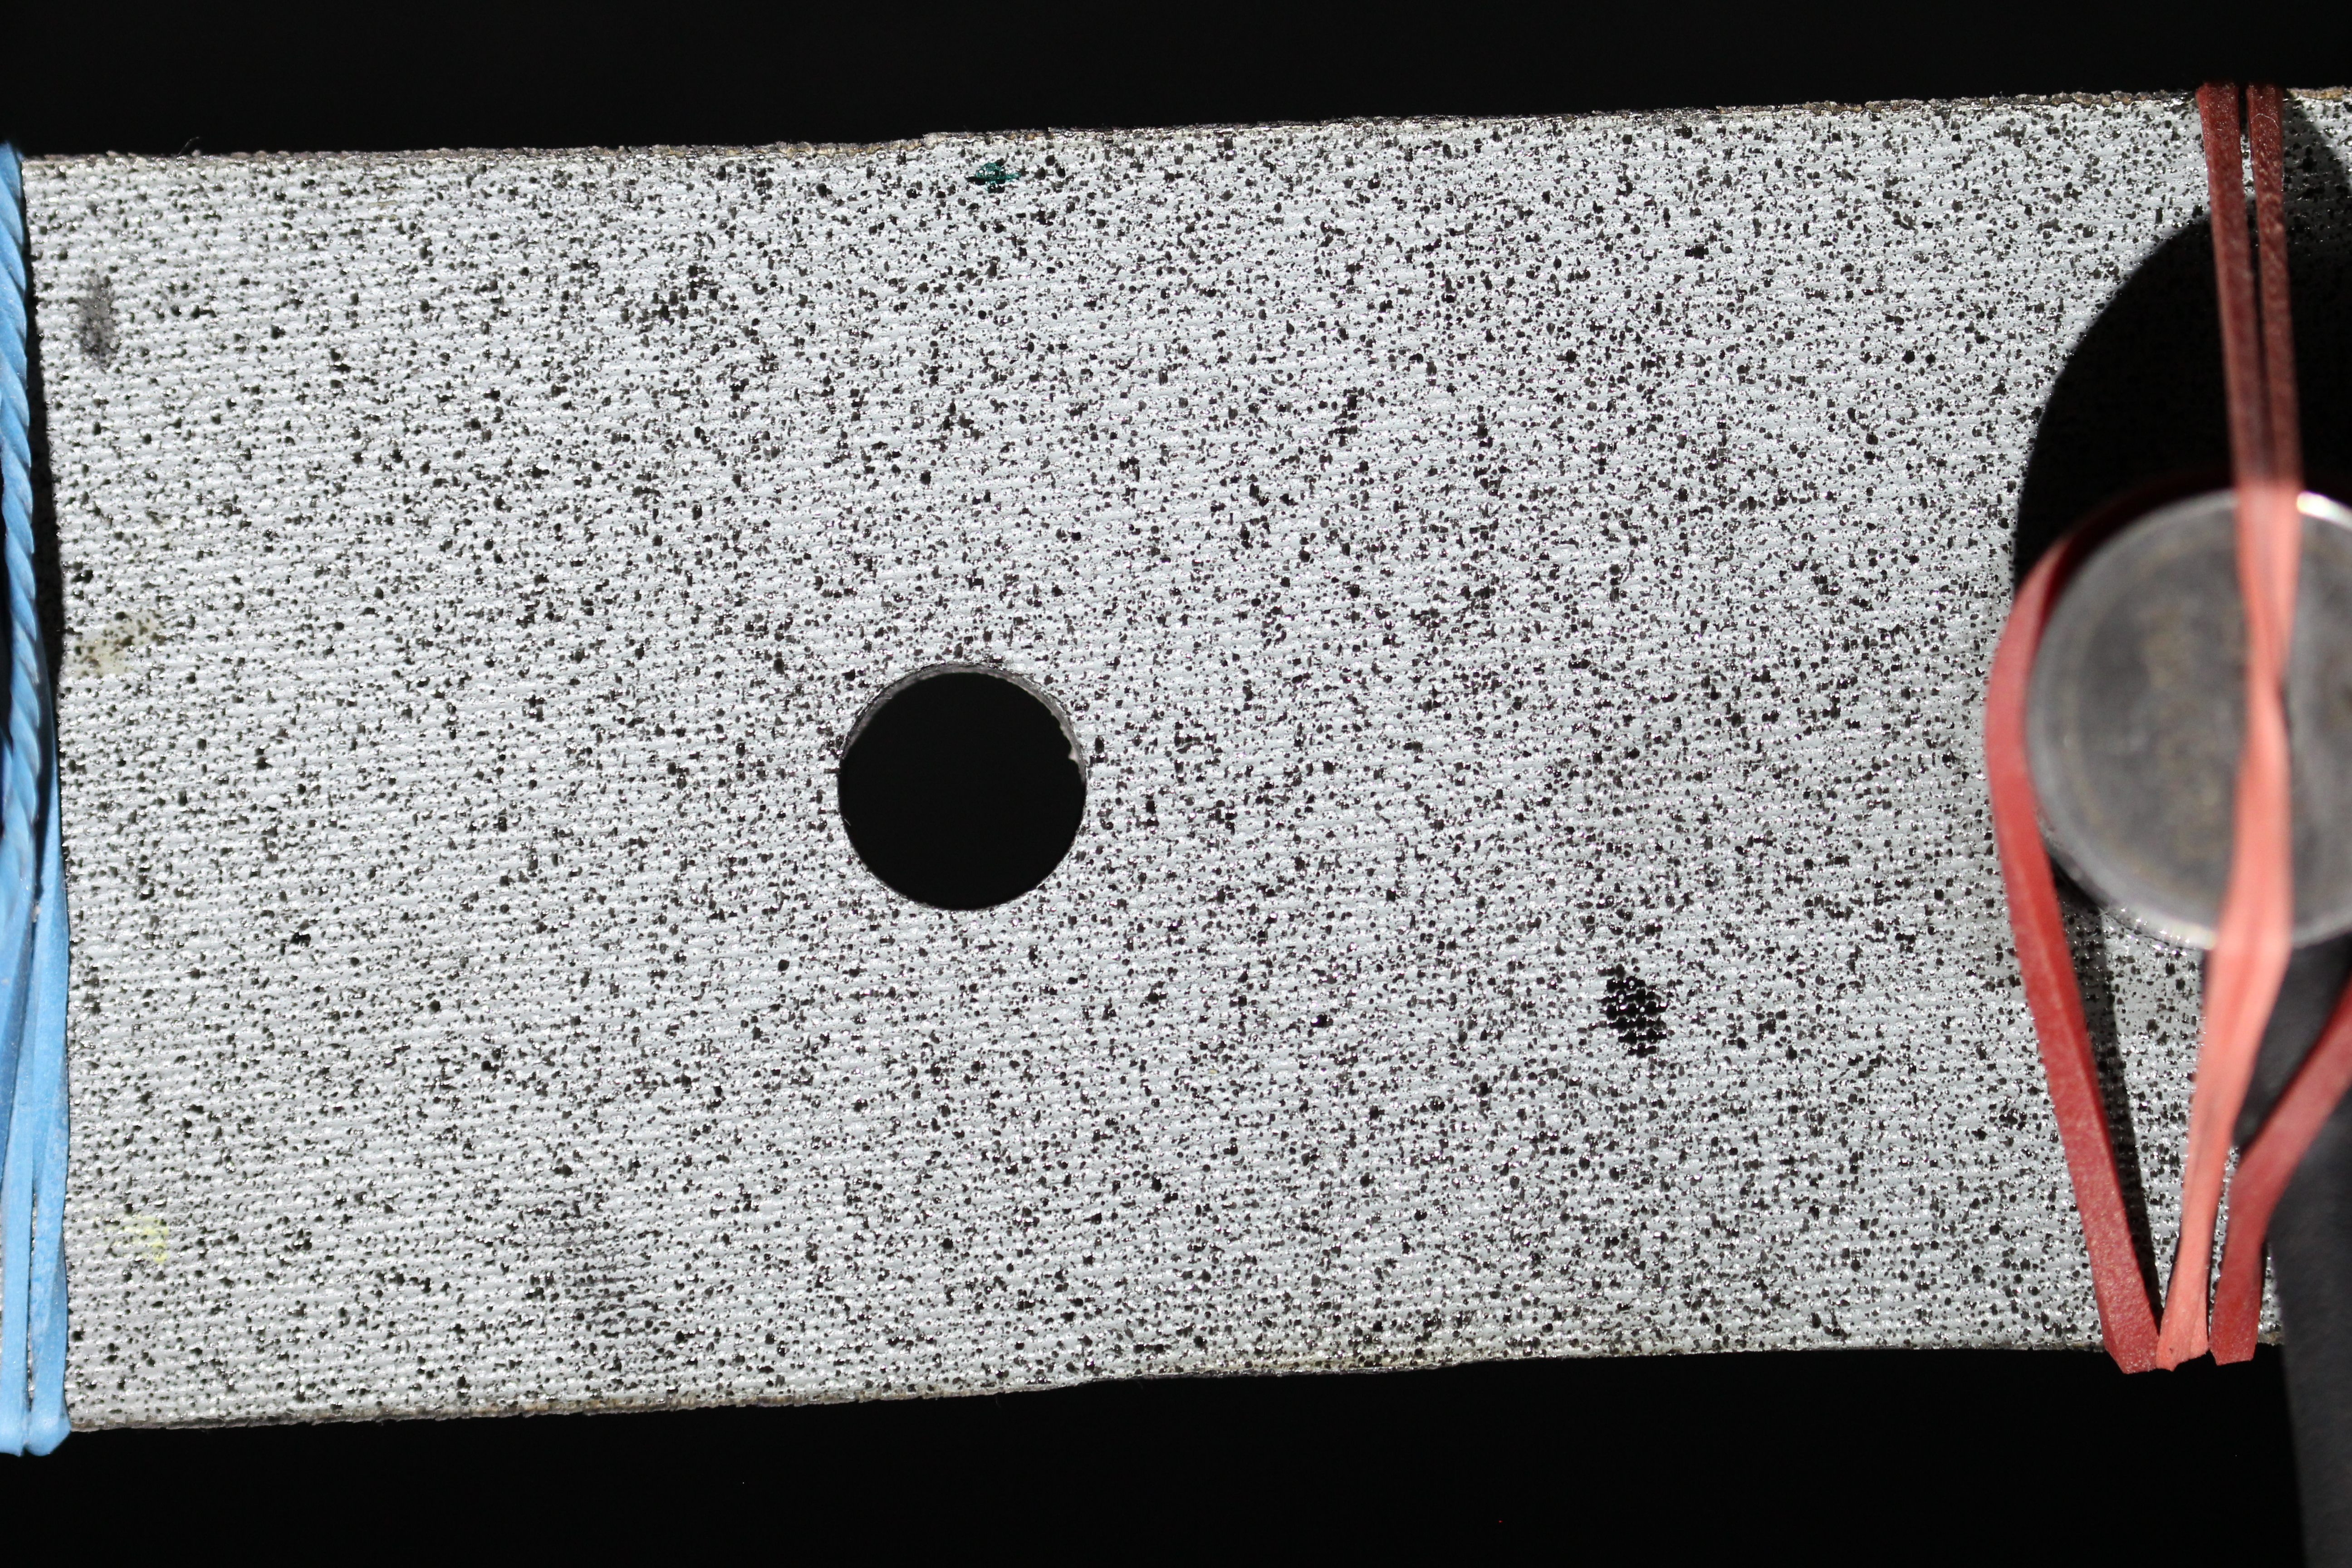
\includegraphics[width=0.6\linewidth]{carbon_deform}}
\caption{Углерод-углеродный композиционный материал}
\label{pic:carbon_deform}
\end{figure}

Фотографирование поверхности осуществляли с помощью фотокамеры Canon EOS 550D, оснащённой длиннофокусным объективом Canon EF-S 100-400mm 1/4-5.6 IS.

\subsection{Тестирование программного обеспечения}
\subsubsection{Тестирование на модельных изображениях}

Для первого раза используем изображения из серии Grey texture, представленные на рисунке \ref{pic:gray_set}. Они имеют сдвиг по оси $x$ на один пиксель влево, по $y$ сдвиг отсутствует.

\begin{figure}[ht]
\center{\includegraphics[width=0.6\linewidth]{gray_set}}
\caption{Тестовая серия изображений: Grey texture}
\label{pic:gray_set}
\end{figure}

Результатом работы ПО, как описано в первом разделе, является векторное поле и поля деформации твёрдого тела представленное на рисунке \ref{pic:gray_set_out}.

\begin{figure}[ht]
\center{\includegraphics[width=0.6\linewidth]{gray_set_out}}
\caption{Поле смещений и деформации твёрдого тела}
\label{pic:gray_set_out}
\end{figure}

\begin{figure}[ht]
\center{\includegraphics[width=0.6\linewidth]{gray_set_func_iteration}}
\caption{Зависимость уровня ошибки, от числа итераций}
\label{pic:gray_set_func_iteration}
\end{figure}

\begin{figure}[ht]
\center{\includegraphics[width=0.6\linewidth]{gray_set_func_iter_vector}}
\caption{Зависимость смещение по x, от числа итераций}
\label{pic:gray_set_func_iter_vector}
\end{figure}

\subsubsection{Тестирование на экспериментально полученных изображения}
В данном разделе приведены результаты тестирования разрабатываемого программного обеспечения на изображениях поверхностей реальных образцов.

\subsection{Исследование метода интерполяции}

\subsection{Исследование размера окна поиска}
